\documentclass[12pt]{article}
\usepackage[left=0.25cm,top=1cm,right=0.25cm,bottom=1cm]{geometry}
\textwidth = 20cm
\hoffset = -1cm
\usepackage[utf8]{inputenc}
\usepackage[spanish,es-tabla]{babel}
\usepackage[autostyle,spanish=mexican]{csquotes}
\usepackage[tbtags]{amsmath}
\usepackage{nccmath}
\usepackage{amsthm}
\usepackage{amssymb}
\usepackage{graphicx}
\usepackage{standalone}
\usepackage[outdir=./]{epstopdf}
\usepackage{siunitx}
\usepackage{physics}
\usepackage{color}
\usepackage{float}
\usepackage{multicol}
%\usepackage{milista}
\usepackage{enumitem}
\usepackage{anyfontsize}
\usepackage{anysize}
\usepackage{enumitem}
\usepackage{capt-of}
\usepackage{bm}
\usepackage{relsize}
\usepackage{placeins}
\usepackage{empheq}
\usepackage{cancel}
\usepackage{wrapfig}
\spanishdecimal{.}
\renewcommand{\baselinestretch}{1.5} 
\renewcommand\labelenumii{\theenumi.{\arabic{enumii}}}
\newcommand{\ptilde}[1]{\ensuremath{{#1}^{\prime}}}
\newcommand{\stilde}[1]{\ensuremath{{#1}^{\prime \prime}}}
\newcommand{\ttilde}[1]{\ensuremath{{#1}^{\prime \prime \prime}}}
\newcommand{\ntilde}[2]{\ensuremath{{#1}^{(#2)}}}


\title{Polinomios de Hermite \\ \large{El oscilador armónico cuántico}} \vspace{-3ex}
\author{M. en C. Gustavo Contreras Mayén}
\date{ }
\newcommand{\Cancel}[2][black]{{\color{#1}\cancel{\color{black}#2}}}
\begin{document}
\vspace{-4cm}
\maketitle
\fontsize{14}{14}\selectfont
\tableofcontents
\newpage

%Referencia: Griffiths - Introduction to quantum mechanics. Cap. 2.3
\section{Introducción.}

Sabemos que el oscilador armónico clásico consiste de una masa $m$ atada a un resorte con una constante $k$, el movimiento que describe la masa sigue la ley de Hooke:
\begin{align*}
F = - k \, x = m \, \dv[2]{x}{t}
\end{align*}

que tiene por solución (si omitimos la fricción)
\begin{align*}
x(t) = A \, \sin (\omega \, t) + B \, \cos (\omega \, t)
\end{align*}

donde
\begin{align}
\omega \equiv \sqrt{\dfrac{k}{m}}
\label{eq:ecuacion_02_036}
\end{align}

es la frecuencia angular de oscilación. La energía potencial correspondiente es
\begin{align}
V(x) = \dfrac{1}{2} k \, x^{2}
\label{eq:ecuacion_02_037}
\end{align}

cuyo trazo es el de una parábola.
\par
De hecho, no existe como tal un oscilador armónico \emph{perfecto}: si estiramos demasiado el resorte, éste se romperá, por lo que la ley de Hooke ya no se cumple una vez que se alcanza este punto.
\par
Podemos considerar que cualquier potencial es \textit{aproximadamente} parabólico en la vecindad de un mínimo local, como se puede ver en la figura (\ref{fig:figura_001}):
\begin{figure}[H]
    \centering
    \includegraphics[scale=0.5]{Imagenes/Potencial_arbitrario.png}
    \caption{Aproximación parabólica (curva sesgada) en un potencial arbitrario, en la vecindad de un mínimo local.}
    \label{fig:figura_001}
\end{figure}

Es posible expandir el potencial $V(x)$ es una serie de Taylor alrededor del mínimo:
\begin{align*}
V(x) = V(x_{0}) + \ptilde{V} (x_{0}) (x - x_{0}) + \dfrac{1}{2} \stilde{V} (x_{0}) (x - x_{0}) + \ldots
\end{align*}

Veamos que:
\begin{enumerate}
\item Es posible eliminar $V(x_{0})$, ya que podemos agregar una constante al potencial $V(x)$ y no modifica en nada a la fuerza.
\item Tenemos que $\ptilde{V}(x_{0}) = 0$, ya que $x_{0}$ es un mínimo local.
\item Podemos descartar los términos de orden superior, que se anulan mientras $(x - x_{0})$ se mantenga pequeño.
\end{enumerate}

Por lo que el potencial se representa como
\begin{align*}
V(x) \cong \dfrac{1}{2} \, \stilde{V} (x_{0}) (x - x_{0})^{2}
\end{align*}

que describe un oscilación armónica (alrededor de $x_{0}$), con una constante efectiva del resorte $k = \stilde{V} (x_{0}$).\footnote{Considera que $\stilde{V}(x_{0})\geq 0$, tomando en cuenta de que $x_{0}$ es un mínimo local. En el extraño caso de que $\stilde{V} (x_{0})= 0$, la oscilación ya no se aproxima a la de un oscilador armónico.}
\par
Esta es la importancia del oscilador armónico: cualquier movimiento oscilatorio se puede aproximar a una oscilación armónica, mientras la amplitud sea pequeña.

\section{El problema cuántico.}

El problema cuántico es resolver la ecuación de Schrödinger para el potencial
\begin{align}
V(x) = \dfrac{1}{2} m \, \omega^{2} \, x^{2}
\label{eq:ecuacion_02_038}
\end{align}

Por lo que la ecuación de Schrödinger independiente del tiempo es
\begin{align}
- \dfrac{\hbar}{2 m} \dv[2]{\psi}{x} + \dfrac{1}{2} m \, \omega \, x^{2} \, \psi = E \, \psi
\label{eq:ecuacion_02_039}
\end{align}

En la literatura se encontrarán dos enfoques completamente diferentes para resolver este problema. El primero es una solución de \enquote{fuerza bruta} directa a la ecuación diferencial, que utiliza el método de expansión en una serie de potencias; tiene la virtud de que la misma estrategia se puede aplicar a muchos otros potenciales. El segundo es una técnica algebraica \emph{ingeniosa}, que utiliza los llamados \textbf{operadores de escalera}.
\par
Primero mostraremos el método algebraico, porque es más rápido y simple (y más divertido).

\subsection{Método algebraico.}

Antes de iniciar, vamos a escribir la ec. (\ref{eq:ecuacion_02_039}) de una manera más sugestiva:
\begin{align}
\dfrac{1}{2 m} \left[ \left( \dfrac{\hbar}{i} \dv{x} \right)^{2} + (m \, \omega \, x)^{2} \right] \, \psi = E \, \psi
\label{eq:ecuacion_02_040}
\end{align}

La idea es factorizar los términos dentro de los corchetes. Si éstos fueran números, podríamos hacerlo fácilmente, ya que
\begin{align*}
u^{2} + v^{2} = (u - i \, v)(u + i \, v)
\end{align*}

Pero no del todo es simple, ya que $u$ y $v$ son \textbf{operadores}, y los operadores en general, \textit{no conmutan} ($u \, v$ no es lo mismo que $v \, u$). Aún así, veamos la siguiente expresión:
\begin{equation}
a_{\pm} \equiv \dfrac{1}{\sqrt{2 m }} \left( \dfrac{\hbar}{i} \dv{x} \pm i \, m \, \omega \, x \right)
\label{eq:ecuacion_02_041}
\end{equation}

¿Cuál es el producto de $a_{-} \, a_{+}$? \emph{Advertencia}: los operadores pueden ser complicados para trabajar en concreto con ellos, y estamos obligados a cometer errores a menos que le asignemos una \enquote{función de prueba}, $f (x)$, para que actúen. Al final, podemos deshacernos de la función de prueba y quedaremos con una ecuación que involucra sólo a los operadores. En nuestro caso del oscilador cuántico, tenemos:
\begin{align*}
a_{-} \, a_{+} f(x) &= \dfrac{1}{2 m} \left( \dfrac{\hbar}{i} \dv{x} - i \, m \, \omega \, x \right) \left( \dfrac{\hbar}{i} \dv{x} + i \, m \, \omega \, x \right) \, f(x) \\[1em]
&= \dfrac{1}{2 m} \left( \dfrac{\hbar}{i} \dv{x} - i \, m \, \omega \, x \right) \left( \dfrac{\hbar}{i} \dv{f}{x} + i \, m \, \omega \, x \, f \right) \\[1em]
&= \dfrac{1}{2 m}  \left[ - \hbar^{2} \dv[2]{f}{x} + \hbar \, m \, \omega \dv{x} (x \, f) - \hbar \, m \, \omega \, x \, \dv{f}{x} + (m \, \omega \, x)^{2} \, f \right] \\[1em]
&= \dfrac{1}{2 m} \left[ \left( \dfrac{\hbar}{i} \dv{x} \right)^{2} + (m \, \omega \, x)^{2} + \hbar \, m\, \omega \right] \, f(x)
\end{align*}

En el último paso hemos utilizado
\begin{align*}
\dv{x} (x \, f) = x \left( \dv{f}{x} \right) + f
\end{align*}

Retirando la función de prueba, llegamos a que
\begin{align}
a_{-} \, a_{+} = \dfrac{1}{2 m} \left[ \left( \dfrac{\hbar}{i} \dv{x} \right)^{2} + (m \, \omega \, x)^{2} \right] + \dfrac{1}{2} \hbar \, \omega
\label{eq:ecuacion_02_042}
\end{align}

Es claro que la ec. (\ref{eq:ecuacion_02_040}) no es factorizable de una manera perfecta, ya que hay un término adicional: $(1/2) \hbar \, \omega$. De todos modos, si ponemos este extra en el otro lado de la ecuación de Schrödinger, tenemos que
\begin{align}
(a_{-} \, a_{+} - \dfrac{1}{2} \hbar \, \omega) \, \psi = E \, \psi
\label{eq:ecuacion_02_43}
\end{align}

Es importante considerar que el orden de los factores $a_{+}$ y $a_{-}$ es importante, con el mismo argumento con $a_{+}$ en la izquierda, llegamos a
\begin{align}
a_{+} \, a_{-} = \dfrac{1}{2 m} \left[ \left( \dfrac{\hbar}{i} \dv{x} \right)^{2} + (m \, \omega \, x)^{2} \right] - \dfrac{1}{2} \hbar \, \omega
\label{eq:ecuacion_02_044}
\end{align}

Por lo tanto
\begin{align}
a_{-} \, a_{+} - a_{+} \, a_{-} = \hbar \, \omega
\label{eq:ecuacion_02_045}
\end{align}

y la ecuación de Schrödinger se puede escribir como
\begin{align}
(a_{+} \, a_{-} + \dfrac{1}{2} \hbar \, \omega) \, \psi = E \, \psi
\label{eq:ecuacion_02_046}
\end{align}

Ahora, aquí viene el paso crucial: \emph{afirmamos que si $\psi$ cumple con la ecuación de Schrödinger, con la energía $E$, entonces $a_{+} \, \psi$ satisface la ecuación de Schrödinger con la energía $(E + \hbar \omega)$}.
\par
Demostración:
\begin{align*}
(a_{+} \, a_{-} + \dfrac{1}{2} \hbar \, \omega) (a_{+} \, \psi) &= \left( a_{+} \, a_{-} \, a_{+} + \dfrac{1}{2} \hbar \, \omega \, a_{+} \right) \psi = \\
&= a_{+} \left( a_{-} \, a_{+} + \dfrac{1}{2} \hbar \, \omega \right) \, \psi = \\
&= a_{+} \left[ \left( a_{-} \, a_{+} - \dfrac{1}{2} \hbar \, \omega \right) \, \psi + \hbar \, \omega \, \psi \right] \\
&= a_{+} (E \, \psi + \hbar \, \omega \, \psi) = \\
&= (E + \hbar \, \omega) (a_{+} \, \psi) \qed
\end{align*}

Observése que mientras que el orden de $a_{+}$ y de $a_{-}$ sí importa, el ordenamiento de $a_{\pm}$ y cualquier constante (como $\hbar$, $\omega$, y $E$) no importa tanto. De la misma manera, $a_{-} \, \psi$ es una solución con energía $(E - \hbar \, \omega)$:
\begin{align*}
(a_{-} \, a_{+} - \dfrac{1}{2} \hbar \, \omega) (a_{-} \, \psi) &= a_{-} \left( a_{+} \, a_{-} - \dfrac{1}{2} \hbar \, \omega \right) \, \psi = \\
&= a_{-} \left[ \left( a_{+} \, a_{-} + \dfrac{1}{2} \hbar \, \omega \right) \, \psi - \hbar \, \omega \, \psi \right] \\
&= a_{-} (E \, \psi - \hbar \, \omega \, \psi) = \\
&= (E - \hbar \, \omega) (a_{-} \, \psi) \qed
\end{align*}

Aquí, entonces, tenemos una \enquote{máquina} maravillosa para extraer nuevas soluciones, con energías más altas y más bajas, ¡si podemos encontrar una solución, para comenzar!
\par
Llamamos a los $a_{\pm}$ \textbf{operadores de escalera}, porque nos permiten subir y bajar en energía:
\begin{itemize}
\item $a_{+}$ se llama operador de subida (o de creación).
\item $a_{-}$ se llama operador de bajada (o de aniquilación) 
\end{itemize}

La \enquote{escalera} de estados se ilustra en la figura (\ref{fig:figura_002}).
\begin{figure}[H]
    \centering
    \includegraphics[scale=0.7]{Imagenes/Operadores_escalera.png}
    \caption{Escalera de estados estacionarios para el oscilador armónico.}
    \label{fig:figura_002}
\end{figure}

¡Pero espera! ¿Qué pasa si aplicamos el operador de bajada repetidamente? ¡Eventualmente llegaremos a un estado con una energía menor que cero, que no existe! En algún momento la máquina debe fallar. ¿Cómo puede suceder eso? 
\par
Sabemos que $a_{-} \psi$ es una nueva solución para la ecuación de Schrödinger, pero \emph{no hay garantía de que sea normalizable}, podría ser cero o su integral cuadrada podría ser infinita. Conclusión: Debe presentarse un \enquote{peldaño más bajo} (llamémoslo $\psi_{0}$) tal que
\begin{align}
a_{-} \, \psi_{0} = 0
\label{eq:ecuacion_02_047}
\end{align}

Es decir
\begin{align*}
\dfrac{1}{\sqrt{2 m}} \left( \dfrac{\hbar}{i} \, \dv{\psi_{0}}{x} - i \, m \, \omega \, x \, \psi_{0} \right) = 0
\end{align*}

o
\begin{align*}
\dv{\psi}{x} = -\dfrac{m \, \omega}{\hbar} \, x \, \psi_{0}
\end{align*}

La ED para $\psi_{0}$ es fácil de resolver
\begin{align*}
\int \dfrac{\dd{\psi_{0}}}{\psi_{0}} = - \dfrac{m \, \omega}{\hbar} \int x \dd{x} \hspace{0.5cm} \Longrightarrow \hspace{0.5cm} \ln \psi_{0} = - \dfrac{m \, \omega}{2 \, \hbar} \, x^{2} + \text{ constante}
\end{align*}

entonces
\begin{align}
\psi_{0} (x) = A_{0} \, \exp \left( - \dfrac{m \, \omega}{2 \, \hbar} x^{2} \right)
\label{eq:ecuacion_02_048}
\end{align}

Para conocer la energía en este estado, usamos este resultado en la ecuación de Schrödinger (en la forma de la ec. (\ref{eq:ecuacion_02_046})) $a_{+} \, a_{-} + (1/2) \hbar \omega = E_{0} \, \psi_{0}$ y aprovechamos el hecho de que $a_{-} \, \psi_{0} = 0$. Por lo que
\begin{align}
E_{0} = \dfrac{1}{2} \hbar \, \omega
\label{eq:ecuacion_02_049}
\end{align}

Ahora con nuestro pie firmemente plantado en el \enquote{peldaño inferior}\footnote{Toma en cuenta que solo puede haber una escalera, ya que el estado más bajo está determinado únicamente por la ec. (\ref{eq:ecuacion_02_047}). Así, de hecho, se han obtenido todas las soluciones (normalizables).} (el estado fundamental del oscilador cuántico, o de energía cero), simplemente aplicamos el operador de subida para generar los estados excitados\footnote{ En el caso del oscilador armónico, es conveniente apartarse de la costumbre habitual y numerar los estados que comienzan con $n = 0$ en lugar de $n = 1$.}
\begin{align}
\setlength{\fboxsep}{3\fboxsep}\boxed{ \psi_{n} (x) = A_{n} \, (a_{+})^{n} \, \exp \left( - \dfrac{m \, \omega}{2 \, \hbar} x^{2} \right) \hspace{1.25cm} E = \left( n + \dfrac{1}{2} \right) \hbar \, \omega}
\label{eq:ecuacion_02_050}
\end{align}

Este método no determina de manera automática la normalización del factor $A_{n}$. Por ejemplo, para calcular $\psi_{1}$, ocupamos el resultado para obtener:
\begin{align*}
\psi_{1} &= A_{1} \, a_{+} \, \exp \left( - \dfrac{m \, \omega}{2 \, \hbar} x^{2} \right) = \\[1em]
&= A_{1} \, \dfrac{1}{\sqrt{2 m}} \left( \dfrac{\hbar}{i} \, \dv{x} + i \, m \, \omega \, x \right) \, \exp \left( - \dfrac{m \, \omega}{2 \, \hbar} x^{2} \right) = \\[1em]
&= \dfrac{A_{1}}{\sqrt{2 m}} \left[ \dfrac{\hbar}{i} \, \left( - \dfrac{m \, \omega}{\hbar} x \right)  \, \exp \left( - \dfrac{m \, \omega}{2 \, \hbar} x^{2} \right) + i \, m \, \omega \, x \, \exp \left( - \dfrac{m \, \omega}{2 \, \hbar} x^{2} \right) \right] 
\end{align*}

que se simplifica como
\begin{align}
\psi_{1} (x) = \left( i \, A_{1} \, \omega \, \sqrt{2 m} \right) \, x \, \exp \left( - \dfrac{m \, \omega}{2 \, \hbar} x^{2} \right)
\label{eq:ecuacion_02_051}
\end{align}

No quisiéramos calcular $\psi_{50}$ de esta manera, pero no importa: hemos encontrado todas las energías permitidas y en principio, hemos determinado los estados estacionarios, el resto es solo cálculo.

\subsection{Método analítico.}

Regresamos nuevamente a la ecuación de Schrödinger para el oscilador armónico (ec. \ref{eq:ecuacion_02_039})
\begin{align*}
- \dfrac{\hbar}{2 m} \dv[2]{\psi}{x} + \dfrac{1}{2} m \, \omega \, x^{2} \, \psi = E \, \psi  
\end{align*}

Para un desarrollo más claro, hacemos el siguiente cambio de variable adimensional
\begin{align}
\xi \equiv \sqrt{ \dfrac{m \omega}{\hbar}} \, x
\label{eq:ecuacion_02_055}
\end{align}

por lo que en términos de $\xi$, la ecuación de Schrödinger toma la forma
\begin{align}
\dv[2]{\psi}{\xi} = (\xi^{2} - K) \, \psi
\label{eq:ecuacion_02_056}
\end{align}

donde $K$ es la energía, en unidades de $(1/2) \hbar \omega$:
\begin{align}
K = \equiv \dfrac{2 \, E}{\hbar \, \omega}
\label{eq:ecuacion_02_057}
\end{align}

Nuestro problema es resolver la ec. (\ref{eq:ecuacion_02_056}), y durante el proceso obtener los valores \enquote{permitidos} de $K$ (y por tanto de $E$).
\par
Para iniciar, veamos que para valores muy grandes de $\xi$ (que a la vez, es decir que tendríamos valores muy grandes de $x$), el término $\xi^{2}$ domina sobre la constante $K$, por lo que tendríamos
\begin{align}
\dv[2]{\psi}{\xi} \approx \xi^{2} \, \psi
\label{eq:ecuacion_02_058}
\end{align}

que tiene por solución
\begin{align}
\psi (\xi) \approx A \, \exp \left( - \dfrac{\xi^{2}}{2} \right) + B \, \exp \left( + \dfrac{\xi^{2}}{2} \right)
\label{eq:ecuacion_02_059}
\end{align}

en donde encontramos que el término $B$ no se puede normalizar (no funciona cuando $\abs{x} \to \infty$), por lo que las soluciones aceptables con sentido físico, tienen las forma asintótica
\begin{align}
\psi (\xi) = ( \quad ) \exp \left( - \dfrac{\xi^{2}}{2} \right) \hspace{1.5cm} \text{con valores grandes de } \xi
\label{eq:ecuacion_02_060}
\end{align}

Esto sugiere que \enquote{aprovechamos} la parte exponencial,
\begin{align}
\psi (\xi) = h (\xi) \, \exp \left( - \dfrac{\xi^{2}}{2} \right)
\label{eq:ecuacion_02_061}
\end{align}

esperando que lo que queda de $[h (\xi)]$ tenga una forma funcional más simple que $\psi (\xi)$ mismo.\footnote{Toma en cuenta que aunque invocamos algunas aproximaciones para motivar la ec. (\ref{eq:ecuacion_02_061}), lo que sigue es exacto. La técnica para eliminar el comportamiento asintótico es el primer paso estándar en el método de la serie de potencias para resolver ecuaciones diferenciales}
\par
Diferenciando la ec. (\ref{eq:ecuacion_02_061}), se tiene que
\begin{align*}
\dv{\psi}{\xi} = \left( \dv{h}{\xi} - \xi \, h \right) \, \exp \left( - \dfrac{\xi^{2}}{2} \right)
\end{align*}
por lo que la ec. de Schrödinger (ec. \ref{eq:ecuacion_02_056}) es
\begin{align}
\dv[2]{h}{\xi} - 2 \, \xi \, \dv{h}{\xi} +  (K - 1) \, h = 0
\label{eq:ecuacion_02_062}
\end{align}

Proponemos una solución a la ED (\ref{eq:ecuacion_02_062}) en la forma de una serie de potencias en $\xi$:
\begin{align}
h (\xi) = a_{0} + a_{1} \, \xi + a_{2} \, \xi^{2} + \ldots = \sum_{j=0}^{\infty} a_{j} \, \xi^{j}
\label{eq:ecuacion_02_063}
\end{align}

Diferenciamos en dos ocasiones la solución para obtener
\begin{align*}
\dv{h}{\xi} &= \sum_{j=0}^{\infty} j \, a_{j} \, \xi^{j-1} \\
\dv[2]{h}{\xi} &= \sum_{j=0}^{\infty} (j + 1)(j + 2) \, a_{j+2} \, \xi^{j}
\end{align*}

que al sustituir en la ec. (\ref{eq:ecuacion_02_062}), tenemos que
\begin{align}
\sum_{j=0}^{\infty} \bigg[ (j + 1)(j + 2) \, a_{j+2} - 2 \, j \, a_{j} +  (K - 1) \, a_{j} \bigg] \, \xi^{j} = 0
\label{eq:ecuacion_02_64}
\end{align}

Sabemos que los coeficientes para cada potencia de $\xi$ deben de anularse, por tanto
\begin{align*}
(j + 1)(j + 2) \, a_{j+2} - 2 \, j \, a_{j} +  (K - 1) \, a_{j} = 0
\end{align*}

de donde se obtiene que
\begin{align}
a_{j+2} = \dfrac{(2 \, j + 1 - K)}{(j + 1)(j + 2)} \, a_{j}
\label{eq:ecuacion_02_065}
\end{align}

Esta es la \textbf{fórmula de recurrencia}, que es en sí misma, equivalente a la ecuación de Schrödinger. Dado $a_{0}$, podemos obtener $a_{2}, a_{4}, a_{6}, \ldots$, también para un $a_{1}$ dado, podemos obtener los $a_{3}, a_{5}, a_{7}, \ldots$
\par
Podemos escribir entonces:
\begin{align}
h (\xi) = h_{\text{par}} (\xi) + h_{\text{impar}} (\xi)
\label{eq:ecuacion_02_066}
\end{align}
donde

\begin{align*}
h_{\text{par}} (\xi) = a_{0} + a_{2} \, \xi^{2} + a_{4} \, \xi^{4} + \ldots
\end{align*}

si es una función par de $\xi$ (ya que involucra sólo potencias pares) a partir de $a_{0}$, y como
\begin{align*}
h_{\text{impar}} (\xi) = a_{1} \, \xi + a_{3} \, \xi^{3} + a_{5} \, \xi^{5} + \ldots
\end{align*}

si es función impar, a partir de $a_{1}$. Entonces tenemos que la ec. (\ref{eq:ecuacion_02_065}) determina a $h(\xi)$ en términos de dos constantes arbitrarias ($a_{0}$ y $a_{1}$), que es lo que se esperaba, dado que tenemos una ED2.
\par
Aún así, no todas las soluciones que se obtienen son normalizables. Para valores grandes de $j$, la fórmula de recursión pasa a ser (aproximadamente)
\begin{align*}
a_{j+2} \approx \dfrac{2}{j} \, a_{j}
\end{align*}

con una solución (aproximada)
\begin{align*}
a_{j} \approx \dfrac{C}{(j/2)!}
\end{align*}

para alguna constante $C$, y esto nos lleva a (para valores grandes de $\xi$, donde las potencias elevadas dominan)
\begin{align*}
h (\xi) \approx C \sum \dfrac{1}{(j/2)!} \, \xi^{j} \approx C \sum \dfrac{1}{k!} \xi^{2 k} \approx C \, \exp \left( \xi^{2} \right)
\end{align*}

Veamos ahora lo siguiente: si $h \to \exp \left( \xi^{2} \right)$, entonces ¿$\psi \to \exp \left( \xi^{2}/2 \right)$?, por que presenta un comportamiento asintótico que no se desea!
\par
Solo hay una forma de salir de esto: para soluciones normalizables, \textit{la serie de potencias debe terminar}. Debe de presentarse un valor \enquote{mayor} de $j$ (llámalo $n$) de manera que la fórmula de recursión devuelva un $a_{n+2} = 0$ (esto truncará cada una de las series par o impar; la otra debe ser cero desde el principio). Para soluciones físicamente aceptables, entonces, debemos tener que
\begin{align*}
K = 2 \, n + 1
\end{align*}

para un entero positivo $n$, es decir (refiriéndose a la ecuación (\ref{eq:ecuacion_02_057})) que la energía debe ser de la forma
\begin{align}
E_{n} = \left( n + \dfrac{1}{2} \right) \, \hbar \, \omega , \hspace{1.5cm} n = 0, 1, 2, \ldots
\label{eq:ecuacion_02_067}
\end{align}

Así recuperamos, mediante un método completamente diferente, la condición fundamental de cuantificación que encontramos algebraicamente en la ec. (\ref{eq:ecuacion_02_050}).
\par
Para los valores permitidos de $K$, la fórmula de recurrencia es
\begin{align}
a_{j+2} = - \dfrac{2 (n - j)}{(j + 1)(j + 2)} \, a_{j}
\label{eq:ecuacion_02_068}
\end{align}

Si $n = 0$, hay sólo un término en la serie (debemos de escoger $a_{1} = 0$ para cancelar $h_{\text{impar}}$ y $j=0$ en la ec. (\ref{eq:ecuacion_02_068}), nos lleva a $a_{2}=0$)
\begin{align*}
h_{0} (\xi) = a_{0}
\end{align*}

y por lo tanto
\begin{align*}
\psi_{0} (\xi) = a_{0} \, \exp \left( - \dfrac{\xi^{2}}{2} \right)
\end{align*}

que es la ec. (\ref{eq:ecuacion_02_048}).
\par
Para $n=1$, escogemos $a_{0} = 0$ y la ec. (\ref{eq:ecuacion_02_068}) con $j = 1$, nos devuelve $a_{3} = 0$, así
\begin{align*}
h_{1} (\xi) = a_{1} \, \xi
\end{align*}

por lo que
\begin{align*}
\psi_{1} (\xi) = a_{1} \, \xi \, \exp \left( - \dfrac{\xi^{2}}{2} \right)
\end{align*}

que confirma la ec. (\ref{eq:ecuacion_02_051}).
\par
Para $n = 2$, $j = 0$, tenemos que $a_{2} = - 2 \, a_{0}$ y $j = 2$ nos da que $a_{4} = 0$ por lo tanto
\begin{align*}
h_{2} (\xi) = a_{0} (1 - 2 \, \xi^{2})
\end{align*}

y entonces
\begin{align*}
\psi_{2} (\xi) = a_{0} (1 - 2 \, \xi^{2}) \, \exp \left( - \dfrac{\xi^{2}}{2} \right)
\end{align*}

y así sucesivamente.
\par
En general, $h_{n} (\xi)$ será un polinomio de grado $n$ en $\xi$, que involucra sólo las potencias pares, si $n$ es un entero par, y las potencias impares solamente, si $n$ es un entero impar. Aparte del factor global $(a_{0}$ o $a_{1})$, se tienen los llamados \textbf{polinomios de Hermite}, $H_{n} (\xi)$.
\par
Los primeros polinomios de Hermite se muestran en la tabla (\ref{tabla_001}).
%\begin{center}
\begin{table}[H]
\centering
\large
\begin{tabular}{l l}
$H_{0} =$ & $1$ \\
$H_{1} =$ & $2 \, x$ \\
$H_{2} =$ & $4 \, x^{2} - 2 $ \\
$H_{3} =$ & $8 \, x^{3} - 12 \, x$ \\
$H_{4} =$ & $16 \, x^{4} - 48 \, x^{2} + 12 $ \\
$H_{5} =$ & $32 \, x^{5} - 160 \, x^{3} + 120 \, x $
\end{tabular}
\caption{Primeros polinomios de Hermite $H_{n}(x)$.}
\label{tabla_001}
\end{table}

\begin{figure}[H]
    \centering
    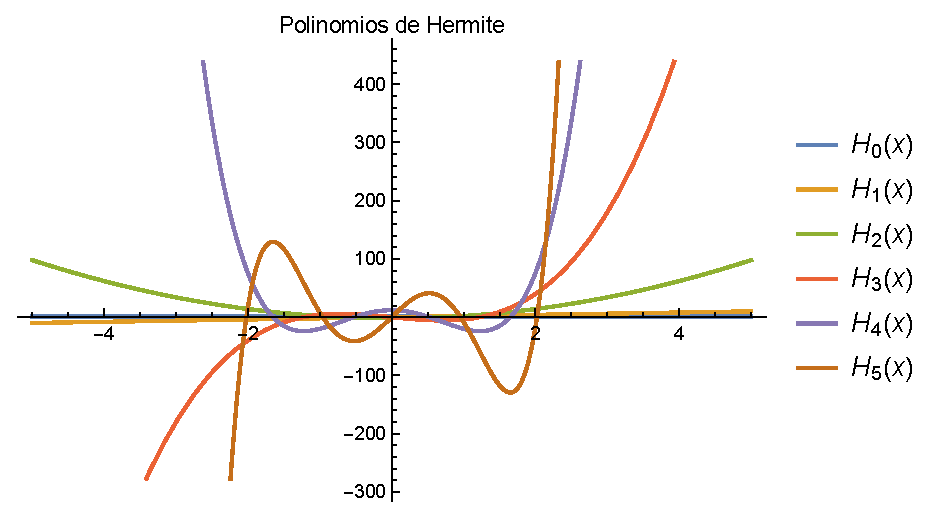
\includegraphics[scale=1.3]{Imagenes/Plot_Hermite.eps}
    \caption{Gráfica de los primeros polinomios de Hermite.}
    \label{figura_003}
\end{figure}
%\end{center}
Por tradición, el factor multiplicativo arbitrario se elige de modo que el coeficiente de la potencia más alta de $\xi$ es $2^{n}$. Con esta convención, los estados estacionarios normalizados para el oscilador armónico son
\begin{align}
\psi_{n} (x) = \left( \dfrac{m \, \omega}{\pi \, \hbar} \right)^{1/4} \, \dfrac{1}{\sqrt{2^{n} \, n!}} \, H_{n} (\xi) \, \exp \left( - \dfrac{\xi^{2}}{2} \right)
\label{eq:ecuacion_02_069}
\end{align}

Son idénticos (por supuesto) a los que obtuvimos algebraicamente en la ec. (\ref{eq:ecuacion_02_050}).
\newpage
En las siguientes figuras, se han trazado la función $\psi_{n} (x)$ para las primeras $n$'s y su normalización.
\begin{figure}[H]
    \centering
    \includegraphics[scale=0.6]{Imagenes/Funcion_Onda_00.eps}
    \includegraphics[scale=0.6]{Imagenes/Funcion_Onda_01.eps}
\end{figure}
\begin{figure}[H]
    \centering
    \includegraphics[scale=0.6]{Imagenes/Funcion_Onda_02.eps}
    \includegraphics[scale=0.6]{Imagenes/Funcion_Onda_03.eps}
\end{figure}
\begin{figure}[H]
    \centering
    \includegraphics[scale=0.6]{Imagenes/Funcion_Onda_04.eps}
    \includegraphics[scale=0.6]{Imagenes/Funcion_Onda_05.eps}
\end{figure}
\begin{figure}[H]
    \centering
    \includegraphics[scale=0.6]{Imagenes/Funcion_Onda_011.eps}
    \includegraphics[scale=0.6]{Imagenes/Funcion_Onda_012.eps}
\end{figure}
\newpage
En la siguiente gráfica se han superpuesto el potencial parabólico y las funciones de onda normalizadas, esquemáticamente representa la solución a la ecuación de Schrödinger.
\begin{figure}[H]
    \centering
    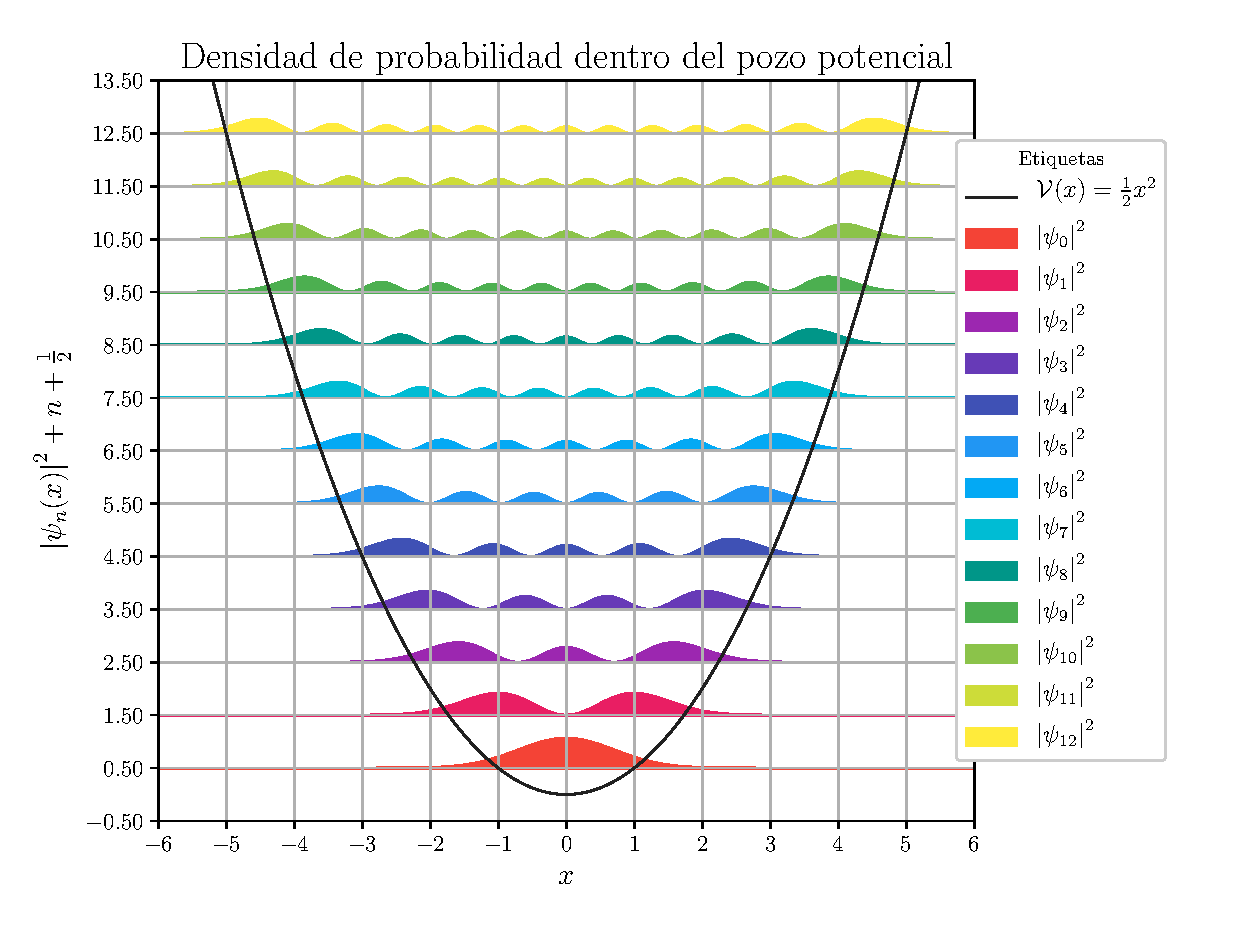
\includegraphics[scale=0.75]{Imagenes/Funciones_Normalizadas_01.eps}
\end{figure}

\newpage

El oscilador cuántico es para sorpresa, muy diferente de su contraparte clásica: no solo se cuantifican las energías, sino que las distribuciones de posición tienen algunas características extrañas. 
\par
Por ejemplo, la probabilidad de encontrar la partícula fuera del rango permitido clásicamente (es decir, con $x$ mayor que la amplitud clásica para la energía en cuestión) no es cero, y en todos los estados impares la probabilidad de encontrar la partícula en el centro del pozo de potencial es cero. Sólo para valores relativamente grandes de $n$ empezamos a ver alguna semejanza con el caso clásico. 
\begin{figure}[H]
    \centering
    \includegraphics[scale=0.5]{Imagenes/Funcion_Onda_100.png}
    \caption{Gráfica para la función de onda $\abs{\psi_{100}}^{2}$, junto con una distribución clásica (línea punteada).}
    \label{figura_004}
\end{figure}

En la figura (\ref{figura_004}), se han superpuesto la distribución de posición clásica en la cuántica (para $n = 100$); si aplanaramos los bultos, los dos encajarían bastante bien (sin embargo, en el caso clásico estamos hablando de la distribución de posiciones en el tiempo para un oscilador, mientras que en el caso cuántico estamos hablando de la distribución en un conjunto de sistemas preparados de manera idéntica).

\section{Propiedades de los Polinomios de Hermite.}

La normalización de los polinomios ha sido elegida de modo tal que 
\begin{align*}
H_{0}(x) = 1
\end{align*}

Algunas de las propiedades de los polinomios de Hermite son:

\begin{align*}
H_{n} (x) &= (-)^{n} \, e^{x^{2}} \, \dv[n]{n} \left( e^{-x^{2}} \right) \\[1em]
\end{align*}
que es la fórmula de Rodrigues.
\par
Algunas relaciones de recurrencia para los polinomios de Hermite son:
\begin{align*}
H_{n+1} (x) &= 2 \, x \, H_{n} (x) - 2 \, n \, H_{n-1} (x) \\
\dot{H}_{n} (x) &= 2 \, n \, H_{n-1} \\
H_{n} (x) &= (-)^{n} \, H_{n} (-x) \\
H_{2n} (0) &= (-)^{n} \, \dfrac{(2 \, n)!}{n!} \\
H_{2n+1} (0) &= 0
\end{align*}


\par
La normalización de la integral que determina la condición de ortogonalidad de los polinomios $\left\{ H_{n} (x) \right\}$ puede hacerse utilizando la siguiente identidad, que define la función generatriz de los polinomios de Hermite:
\begin{align*}
\exp \left( -t^{2} + 2 \, x \, t \right) = \sum_{n=0}^{\infty} \dfrac{H_{n} (x) \, t^{n}}{n!}
\end{align*}

se sigue entonces que:
\begin{align*}
\exp \left( -x^{2} \right) \, & \exp \left( -t^{2} + 2 \, x \, t \right) \, \exp \left( -s^{2} + 2 \, x \, s \right) = \\
&= \sum_{n=0}^{\infty} \, \sum_{m=0}^{\infty} \dfrac{e^{-x^{2}}}{n! \, m!} \, t^{n} \, s^{m} \, H_{n} (x) \, H_{m} (x)
\end{align*}

Integrando con respecto a $x$ en el intervalo $(-\infty, \infty)$ y considerando que
\begin{align*}
\exp \left( -x^{2} \right) \, \exp \left( -t^{2} + 2 x t \right) \, &\exp \left( -s^{2} + 2 x s \right) = \\
&= \exp \left( - (x - s - t)^{2} \right) \, \exp \left( 2 s t \right)
\end{align*}

y con el resultado
\begin{align*}
\int_{-\infty}^{\infty} e^{-x^{2}} \, H_{n} (x) \, H_{m} (x) \, \dd{x} = \delta_{m n} \int_{-\infty}^{\infty} e^{-x^{2}} \, H_{n}^{2} (x) \, \dd{x}
\end{align*}

se obtiene:
\begin{align*}
\sum_{n=0}^{\infty} \dfrac{(s \, t)^{n}}{(n!)^{2}} \int_{-\infty}^{\infty} e^{-x^{2}} \, H_{n}^{2} (x) \, \dd{x} = \sqrt{\pi} \, e^{2 s t } = \sqrt{\pi} \, \sum_{n=0}^{\infty} \sum_{n=0}^{\infty} \dfrac{2^{n} \, (s t)^{n}}{n!}
\end{align*}

de donde:
\begin{align*}
\int_{-\infty}^{\infty} e^{-x^{2}} \, H_{n}^{2} (x) \, \dd{x} = 2^{n} \, \sqrt{\pi} \, n!
\end{align*}

En consecuencia, la condición de ortogonalidad es:
\begin{align}
\setlength{\fboxsep}{3\fboxsep}\boxed{ \int_{-\infty}^{\infty} e^{-x^{2}} \, H_{n} (x) \, H_{m} (x) \dd{x} = 2^{n} \, \sqrt{\pi} \, n! \, \delta_{m n} \hspace{1cm} n = 0, 1, 2, \ldots }
\end{align}

El conjunto $\left\{ H_{n }(x) \right\}$ es completo; por tanto cualquier función $f(x)$ definida en el intervalo $(-\infty, \infty)$ puede expandirse en polinomios de Hermite:
\[ f(x) = \sum_{n=0}^{\infty} C_{n} \, H_{n} (x) \]
En forma general puede afirmarse que cualquier función definida en $(-\infty, \infty)$ puede expandirse en cualquier base ortogonal definida en $(-\infty, \infty)$.
\par
Expresar la función en una u otra es cambiar de base: la misma función puede expandirse, por ejemplo, en la base de Hermite $\left\{ H_{n }(x) \right\}$, o en la de Fourier $\left\{ e^{i k x} \right\}$.

\section{La familia de la ecuación de Hermite.}
A partir de la ecuación de Hermite y utilizando la transformación
\begin{align*}
H_{n} (x) = e^{\alpha x^{2}} \, \psi_{n} (\mu), \hspace{2cm} \mu = x^{b}
\end{align*}

se obtiene la primera familia de Hermite
\begin{align*}
&{} b^{2} \, \dv[2]{\psi_{n} (\mu)}{\mu} \, \mu^{2 (b-1)/b} + \dv{\psi_{n}(\mu)}{\mu} \left[ b \, (b-1) \mu^{\frac{b-2}{2}}  + \right. \\
&+\left. 2 \, b \, (2 \, a - 1) \, \mu \right] + \left[ 4 \, a \, (a - 1) \, \mu^{2/b} + 2 \, n + 2 \, a \right] \, \psi_{n} (\mu) = 0
\end{align*}

cuya solución es
\begin{align*}
\psi_{n} (\mu) = e^{-\alpha x^{2}} \, H_{n} (x) = \exp \left( - \dfrac{a x^{2}}{b} \right) \, H_{n} (\mu^{1/b})
\end{align*}

\begin{enumerate}[label=\roman*.)]
\item Con $a = 0, b = 1$, se recupera la ecuación de Hermite.
\item Si $b = 1, a = 1/2$, se obtiene la ecuación de \textbf{Weber-Hermite}:
\begin{align}
\dv[2]{\psi_{n} (x)}{x} + [ 1 + 2 \, n - x^{2} ] \, \psi_{n} (x) = 0
\label{eq:ecuacion_08_65}
\end{align}
\end{enumerate}

Con $\mu = x$ y $\psi_{n} (x) = e^{-x^{2}/2} / H_{n} (x)$. Esta última describe el oscilador armónicos unidimensional en mecánica cuántica. Nótese que la base $\left\{ \psi_{n} (x) \right\}$ es ortonormal.
\end{document}